%%%%%%%%%%%%%%%%%%%%%%%%%%%%%%%%%%%%%%%%%
% Dreuw & Deselaer's Poster
% LaTeX Template
% Version 1.0 (11/04/13)
%
% Created by:
% Philippe Dreuw and Thomas Deselaers
% http://www-i6.informatik.rwth-aachen.de/~dreuw/latexbeamerposter.php
%
% This template has been downloaded from:
% http://www.LaTeXTemplates.com
%
% License:
% CC BY-NC-SA 3.0 (http://creativecommons.org/licenses/by-nc-sa/3.0/)
%
%%%%%%%%%%%%%%%%%%%%%%%%%%%%%%%%%%%%%%%%%

%----------------------------------------------------------fselec------------------------------
%	PACKAGES AND OTHER DOCUMENT CONFIGURATIONS
%----------------------------------------------------------------------------------------

\documentclass[final,hyperref={pdfpagelabels=false, brazil}]{beamer}

\usepackage[T1]{fontenc}
\usepackage[utf8]{inputenc}

\usepackage[orientation=portrait,size=a0,scale=1.4]{beamerposter} % Use the beamerposter package for laying out the poster with a portrait orientation and an a0 paper size

\usetheme{I6pd2} % Use the I6pd2 theme supplied with this template

\usepackage[english]{babel} % English language/hyphenation

\usepackage{amsmath,amsthm,amssymb,latexsym} % For including math equations, theorems, symbols, etc

%\usepackage{times}\usefonttheme{professionalfonts}  % Uncomment to use Times as the main font
%\usefonttheme[onlymath]{serif} % Uncomment to use a Serif font within math environments

\boldmath % Use bold for everything within the math environment

\usepackage{booktabs} % Top and bottom rules for tables

\graphicspath{{figures/}} % Location of the graphics files

\usecaptiontemplate{\small\structure{\insertcaptionname~\insertcaptionnumber: }\insertcaption} % A fix for figure numbering


%----------------------------------------------------------------------------------------
%	TITLE SECTION 
%----------------------------------------------------------------------------------------

\title{\huge Segmenta\c c\~ao e classifica\c c\~ao de Big Data} % Poster title

\author{Gustavo Kendi Tsuji} % Author(s)

\institute{Universidade de São Paulo} % Institution(s)

%----------------------------------------------------------------------------------------
%	FOOTER TEXT
%----------------------------------------------------------------------------------------

\newcommand{\rightfoot}{Criado a partir do modelo de Philippe Dreuw and Thomas Deselaers do site http://www.LaTeXTemplates.com} % Left footer text

\newcommand{\leftfoot}{} % Right footer text

\usepackage{tabularx}
\usepackage{graphicx}
\usepackage{caption}
\usepackage{subcaption}

\usepackage{ragged2e}
 
\let\olditem=\item% 
\renewcommand{\item}{\olditem \justifying}%

%----------------------------------------------------------------------------------------

\begin{document}
\newcolumntype{L}[1]{>{\raggedright\arraybackslash}m{#1}}
\newcolumntype{C}[1]{>{\centering\arraybackslash}m{#1}}
\newcolumntype{R}[1]{>{\raggedleft\arraybackslash}m{#1}}

\addtobeamertemplate{block end}{}{\vspace*{2ex}} % White space under blocks

\begin{frame}[t] % The whole poster is enclosed in one beamer frame

\begin{columns}[t] % The whole poster consists of two major columns, each of which can be subdivided further with another \begin{columns} block - the [t] argument aligns each column's content to the top

\begin{column}{.02\textwidth}\end{column} % Empty spacer column

\begin{column}{.465\textwidth} % The first column

%----------------------------------------------------------------------------------------
%	INTRODUCTION
%----------------------------------------------------------------------------------------
            
\begin{block}{Introdu\c c\~ao}

\begin{itemize}

\item Hoje é possível encontrar mais de 60 trilhões de páginas indexadas pelo Google\cite{GOO01}. Só o Facebook possui \emph{data warehouses} com mais de 300 \emph{petabytes} e um tráfego de mais de 600 \emph{terabytes} diários\cite{FAC01}. Mas o grande desafio já não é o armazenamento desses dados. Extrair conhecimento dessas informações se tornou o aspecto essencial para as empresas. Trata-se de um ativo intangível estratégico que viabiliza o desenvolvimento de novos produtos ou serviços bem como um melhor entendimento sobre comportamento de clientes e funcionamento de processos ou otimização da produção. Este trabalho apresentará uma abordagem para explorar o que é possível desenvolver num contexto de \emph{Big Data} com algoritmos de \emph{Machine Learning}.

\end{itemize}

\end{block}





%----------------------------------------------------------------------------------------
%	MATERIALS
%----------------------------------------------------------------------------------------

%\begin{block}{Materials}

%\begin{columns} % Subdivide the first main column
%\begin{column}{.54\textwidth} % The first subdivided column within the first main column
%\begin{itemize}
%\item Vestibulum nisl, quis euismod velit eros in ligula.
%\begin{itemize}
%\item Cras rhoncus quam et augue convallis in elementum urna tincidunt.
%\end{itemize}
%\item Proin ut vestibulum augue.
%\begin{itemize}
%\item Donec dapibus sagittis neque eu ultrices.
%\end{itemize}
%\end{itemize}
%\end{column}

%\begin{column}{.43\textwidth} % The second subdivided column within the first main column
%\centering
%\begin{figure}
%
\includegraphics[width=0.8\linewidth]{placeholder.jpg}
%\caption{Figure caption}
%\end{figure}
%\end{column}
%\end{columns} % End of the subdivision

%\begin{itemize}
%\item Curabitur sapien ligula, faucibus in feugiat quis, vestibulum a turpis.
%\begin{itemize}
%\item Phasellus quis nunc neque. Suspendisse mauris diam, suscipit non gravida in, placerat id enim. Ut nec ipsum in lectus ultrices sagittis.
%\item Ut nec ipsum in lectus ultrices sagittis.
%\item Phasellus quis nunc neque.
%\end{itemize}
%\end{itemize}

%\end{block}

%----------------------------------------------------------------------------------------
%	METHODS
%----------------------------------------------------------------------------------------

\begin{block}{Metodologia}


\begin{itemize}
\item Realização de experimento quantitativo de segmentação e classificação de dados. Este estudo utilizou uma base disponível no site kaggle\cite{KAGGLE} com mais de 800 mil registros. Ela possui informações de perfil de mutuários a detalhes das transações. Pertence a Loan Club, uma empresa de empréstimos com um sistema online.

\item A análise consiste em:
\begin{itemize}
\item Estudo dos algoritmos de segmentação K Médias (KM) e de classificação Regressão Logística (RL) e Random Forest (RF)
\item Análise descritiva dos clusters gerados pelo KM
\item Comparação da classificação da RL e RF
\end{itemize}
\end{itemize}

\end{block}

%----------------------------------------------------------------------------------------
%	MATHEMATICAL SECTION
%----------------------------------------------------------------------------------------

\begin{block}{Fundamenta\c c\~ao te\'orica}

\begin{itemize}
\item Clusterização
\begin{itemize}
\item O KM é um método de aprendizagem não supervisionado que reune os elementos em grupos baseados na similaridade entre eles.  \cite{MacQueen}. 

\begin{figure}
\centering
\caption{Ilustração da clusterização de uma amostra de 8000 registros}
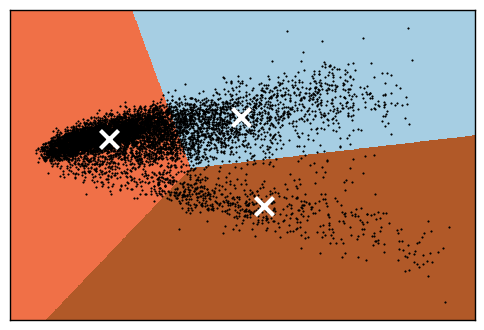
\includegraphics[width=0.65\linewidth]{cluster.png}
\end{figure}

\item Essa similaridade é baseada na minimização da distância Euclidiana entre os vetores de atributos e os centróides dos clusters.

\end{itemize}
\item Classificação
\begin{itemize}
\item A RL é um modelo supervisionado que estuda a relação entre variáveis com o intuito de predizer a ocorrência de eventos. Ao ser treinado, a RL gera uma fórmula que pode classificar dados usando como base o \emph{odd ratios}, isto é, as chances de que um determinado evento ocorra\cite{HASTIE}. 

\begin{equation}
  \label{eq:t}
  \begin{aligned}
    logit^{-1}(\alpha) &= \frac{1}{1+e^{-\alpha}} &= \frac{e^{\alpha}}{1+e^{\alpha}}
  \end{aligned}
\end{equation}

\end{itemize}

\begin{itemize}
\item A RF é um método que gera várias árvores para efetuar a classificação com o intuito de reduzir problemas de viés de usar somente uma. 

\begin{figure}
\caption{Árvore de decisão para a base da Loan Club}
\centering
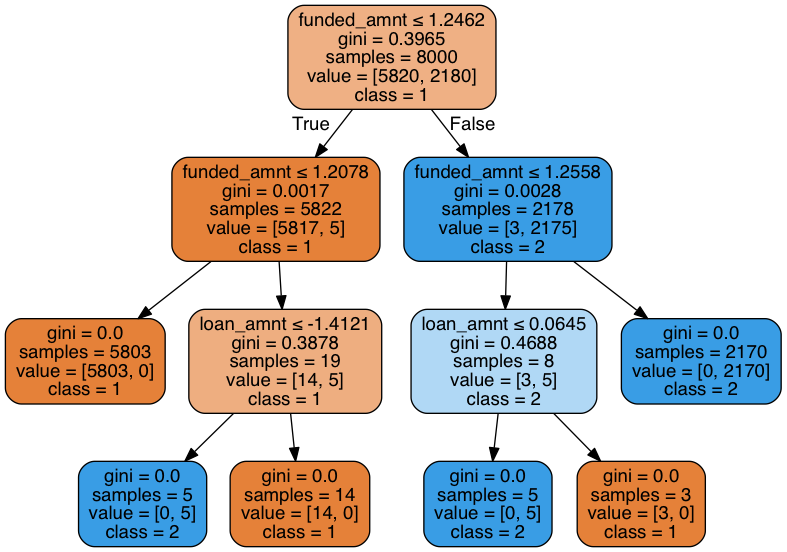
\includegraphics[width=0.66\linewidth]{loan.png}

\end{figure}

\item A árvore de decisão é uma estrutura de modelo preditivo de fácil interpretação utilizado na aprendizagem supervisionada \cite{HASTIE}. Ela define o fluxo que classifica os dados em cada uma de suas extremidades.


\end{itemize}

\end{itemize}

\end{block}

%----------------------------------------------------------------------------------------

\end{column} % End of the first column

\begin{column}{.01\textwidth}\end{column} % Empty spacer column
 
\begin{column}{.465\textwidth} % The second column

%----------------------------------------------------------------------------------------
% OBJECTIVES
%----------------------------------------------------------------------------------------

\begin{block}{Objetivos}

\begin{enumerate}
\item Segmentar e classificar dados usando Scikit Learn\cite{SCI} e Apache Spark\cite{SPARK} 

\end{enumerate}


\end{block}

%----------------------------------------------------------------------------------------
%	RESULTS
%----------------------------------------------------------------------------------------
%\begin{table}
%\begin{tabular}{l l l}
%\toprule
%\textbf{Treatments} & \textbf{Response 1} & \textbf{Response 2}\\
%\midrule
%Treatment 1 & 0.0003262 & 0.562 \\
%Treatment 2 & 0.0015681 & 0.910 \\
%Treatment 3 & 0.0009271 & 0.296 \\
%\bottomrule
%\end{tabular}
%\caption{Table caption}
%\end{table}

%\begin{itemize}
%\item Sollicitudin Vel Orci
%\item Maecenas Ultricies Feugiat Velit Non Mattis.
%\end{itemize}

%\begin{table}
%\begin{tabular}{l l l}
%\toprule
%\textbf{Treatments} & \textbf{Response 1} & \textbf{Response 2}\\
%\midrule
%Treatment 1 & 0.0003262 & 0.562 \\
%Treatment 2 & 0.0015681 & 0.910 \\
%Treatment 3 & 0.0009271 & 0.296 \\
%\bottomrule
%\end{tabular}
%\caption{Table caption}
%\end{table}
     
%\end{block}

%------------------------------------------------

\begin{block}{Resultados}

\begin{itemize}
\item Clusterização

\begin{itemize}
\item Usando o Scikit Learn foi possível visualizar diversas clusterizações. Foi escolhido o particionamento dos dados em 3 grupos.

%\begin{figure}
%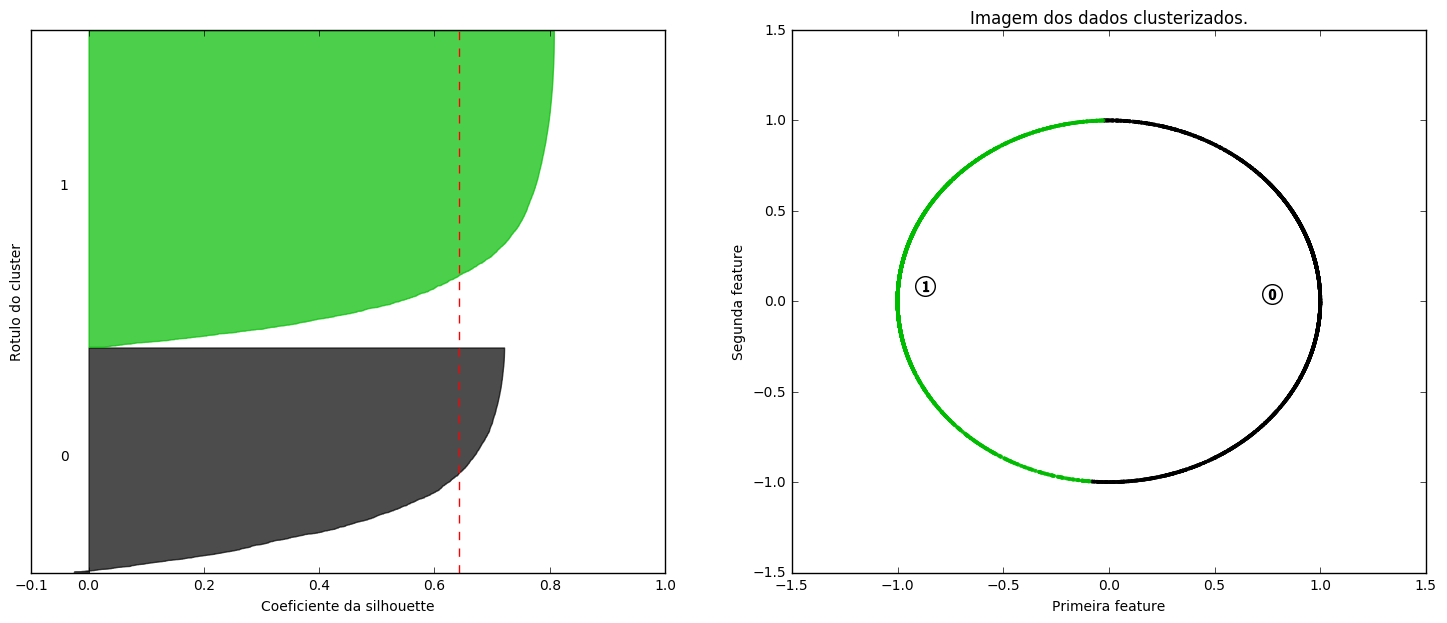
\includegraphics[width=0.85\linewidth]{silhoute2.png}
%\caption{Clusterização}
%\end{figure}

\begin{figure}[t!]
    \centering
        \caption{Resultados da clusterização}
    \begin{subfigure}[t]{0.55\textwidth}
        \centering
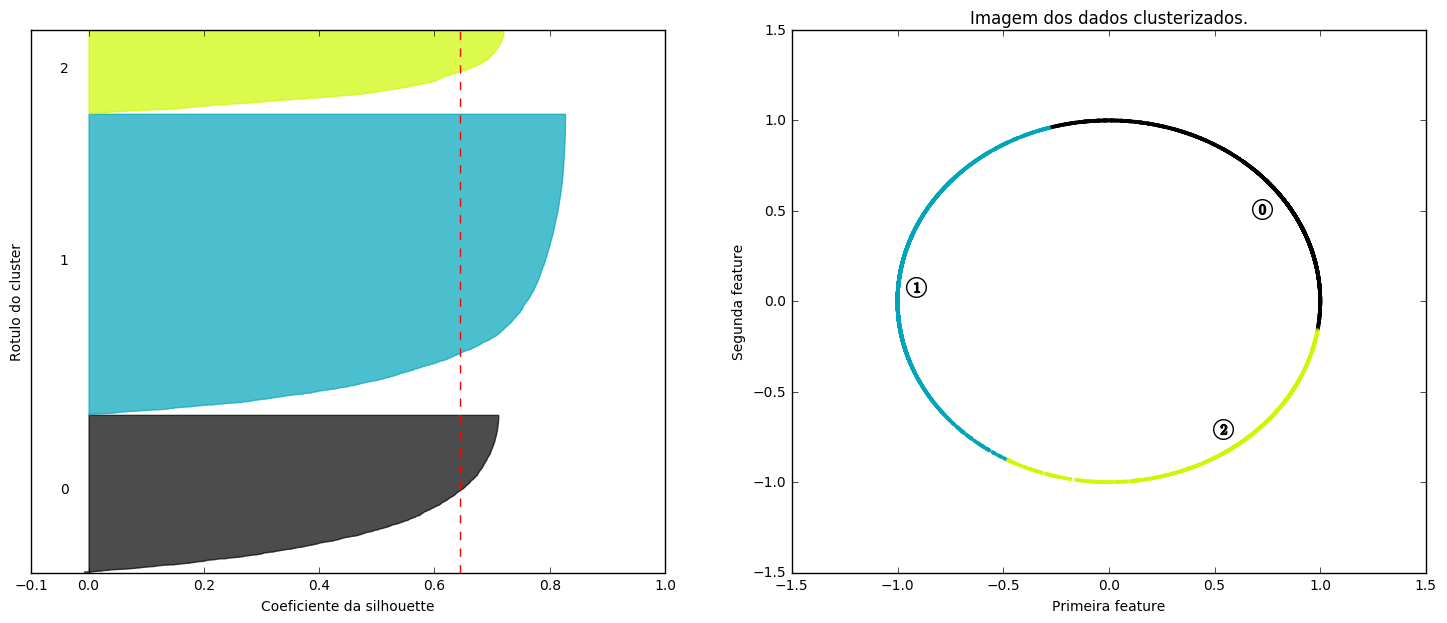
\includegraphics[width=1\linewidth]{silhoute3.png}

        \caption{Ilustração do silhoutte score para 3 clusters}
    \end{subfigure}%
    ~ 
    \begin{subfigure}[t]{0.35\textwidth}
        \centering
        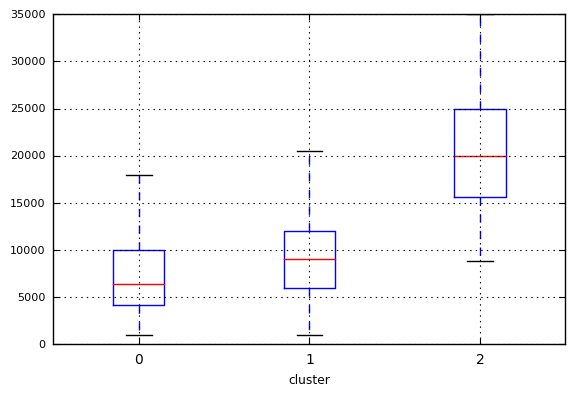
\includegraphics[width=1\linewidth]{loan_amnt_by_cluster.png}
        \caption{Box plot por cluster do campo loan\_amnt\_by\_cluster}
    \end{subfigure}


\end{figure}



\end{itemize}

\end{itemize}

\begin{itemize}
\item Classificação

\begin{itemize}
\item Baseado na clusterização realizada pelo KM, utilizou-se uma \emph{Cross Validation} treinando 80\% da base com RL e RF e classificando os 20\% restantes

\end{itemize}

%\begin{tabular}{ C{3cm} | C{5cm} | C{5cm} | C{5cm} | }

%    \hline 
%    1    & 29585 & 334   & 1307  \\[3ex]
%    \hline
%    2    & 715   & 58836 & 3957  \\[3ex]
%    \hline
%    3    & 1342  & 5006  & 164590 \\[3ex]
%    \hline
    
%\end{tabular}



\begin{itemize}

\item Após o treinamento, gerou-se as Confusion Matrices de cada algoritmo

\begin{figure}[t!]
    \centering
        \caption{Confusion Matrices}
    \begin{subfigure}[t]{0.42\textwidth}
        \centering
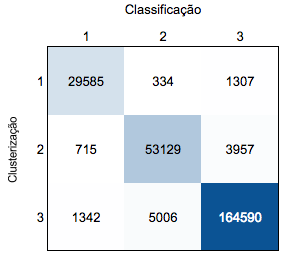
\includegraphics[width=1\linewidth]{CM-RL-abs.png}

        \caption{Confusion Matrix da RL}
    \end{subfigure}%
    ~ 
    \begin{subfigure}[t]{0.43\textwidth}
        \centering
        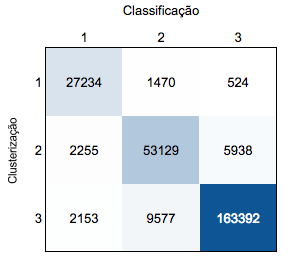
\includegraphics[width=1\linewidth]{CM-RF-abs.png}
        \caption{Confusion matrix da RF}
    \end{subfigure}


\end{figure}

%\begin{tabular}{ r r r r }

%         & 1 & 2 & 3 \\
%    1    & 27234 & 1470   & 524  \\
%    2    & 2255   & 53129 & 5938  \\
%    3    & 2153  & 9577   & 163392
%\end{tabular}



\end{itemize}

\begin{itemize}
\item Pelos estudos, é possível compararmos as métricas de cada classificação e concluimos que a RL teve um melhor resultado.


%\begin{tabular}{@{} *5c @{}}    \toprule
%  Classe & Precisão & Recall  & FP & F-measure  \\\midrule
%    1 & 0,9349 & 0,9474 & 0,0087 & 0,9411 \\
%    2 & 0,9167 & 0,9264 & 0,0264 & 0,9523 \\
%    3 & 0,9690 & 0,9628 & 0,0555 & 0,9524 \\\bottomrule
% \hline
%\end{tabular}



%\begin{tabular}{@{} *5c @{}}    \toprule
%  Classe & Precisão & Recall  & FP & F-measure  \\\midrule
%    1 & 0,8606 & 0,9317 & 0,0186 & 0,8948 \\
%    2 & 0,8278 & 0,8663 & 0,0540 & 0,8466 \\
 %   3 & 0,9619 & 0,9330 & 0,0713 & 0,9472 \\
 %   \bottomrule
% \hline
%\end{tabular}

\begin{table}
\centering
        \caption{Métricas de assertividade e eficiência da RL e da RF}
        \label{multiprogram}
        \begin{tabular}{c | c c | c c | c c|c c } \toprule
             Classe & \multicolumn{2}{|c|}{Precisão} & \multicolumn{2}{|c|}{Recall} & \multicolumn{2}{|c|}{Falso Positivo} & \multicolumn{2}{|c}{F-measure}\\
            \cline{2-9}
             & RL & RF & RL & RF & RL & RF & RL & RF \\
             \hline
            \multicolumn{1}{c|}{1} & 0,9349 & 0,8606 & 0,9474 & 0,9317 & 0,0087 &  0,0186 & 0,9411 & 0,8948\\
            \multicolumn{1}{c|}{2} & 0,9167 & 0,8278 & 0,9264 & 0,8663 & 0,0264 & 0,0540 & 0,9523 & 0,8466\\
            \multicolumn{1}{c|}{3} & 0,9690 & 0,9619 & 0,9628 & 0,9330 & 0,0555 & 0,0713 & 0,9524 & 0,9472\\\bottomrule
        \end{tabular}
    \end{table}


\end{itemize}
\end{itemize}
\end{block}

%----------------------------------------------------------------------------------------
%	CONCLUSION
%----------------------------------------------------------------------------------------

\begin{block}{Conclus\~ao}

\begin{itemize}
\item Ambas ferramentas se mostraram que se complementam: o Scikit Learn possui muitos recursos que facilitam a visualização e a compreensão dos modelos, já o Apache Spark é robusto e eficiente, executando os algoritmos de forma rápida e escalável, ideal para o cenário de Big Data.

\item A segmentação gerou 3 clusters e foi possível observar as diferenças entre si.

\item Na classificação, mesmo com uma menor assertividade, a RF também é um algoritmo com alta eficiência. Possivelmente com outra configuração (redução de cluster, aumento de profundidade ou aumento de árvores) o resultado poderia ser diferente.


\end{itemize}

\end{block}

%----------------------------------------------------------------------------------------
%	REFERENCES
%----------------------------------------------------------------------------------------

\begin{block}{Refer\^encia Bibliogr\'afica}
        
\nocite{*} % Insert publications even if they are not cited in the poster
\scriptsize{\bibliographystyle{acm}
\bibliography{sample}}

\end{block}



%----------------------------------------------------------------------------------------
%	CONTACT INFORMATION
%----------------------------------------------------------------------------------------

%\setbeamercolor{block title}{fg=black,bg=orange!70} % Change the block title color

%\begin{block}{Contact Information}

%\begin{itemize}
%\item Web: \href{http://www.university.edu/smithlab}{http://www.university.edu/smithlab}
%\item Email: \href{mailto:john@smith.com}{john@smith.com}
%\item Phone: +1 (000) 111 1111
%\end{itemize}

%\end{block}

%----------------------------------------------------------------------------------------

\end{column} % End of the second column

\begin{column}{.015\textwidth}\end{column} % Empty spacer column

\end{columns} % End of all the columns in the poster

\end{frame} % End of the enclosing frame

\end{document}